\documentclass{article}
\usepackage{tikz}

\begin{document}
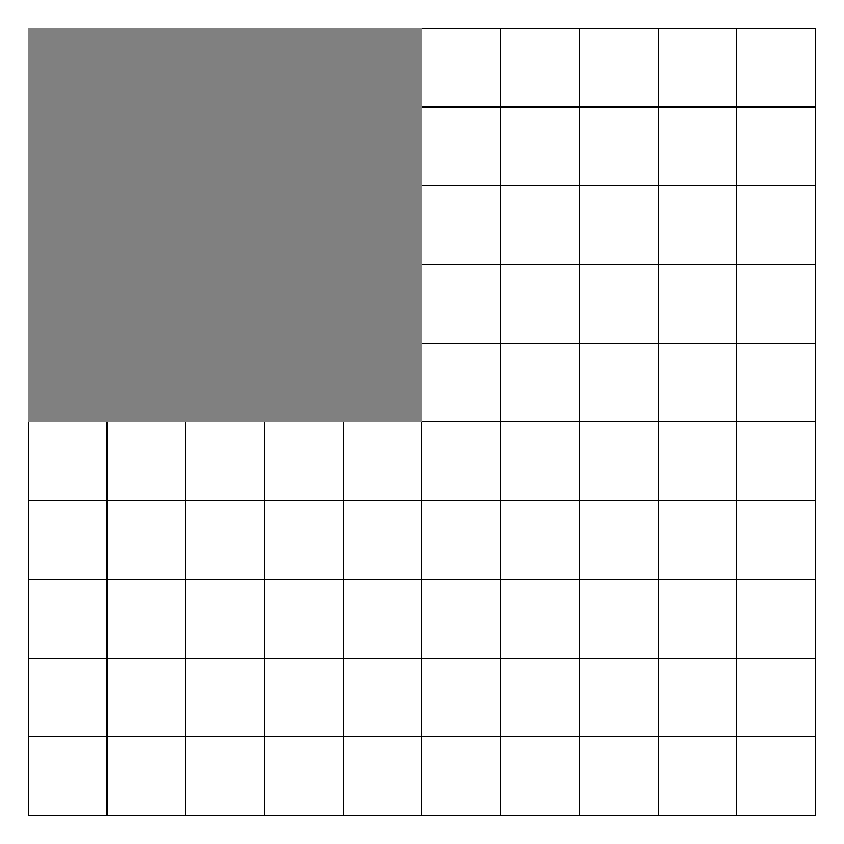
\begin{tikzpicture}
% Draw a 10x10 grid
\draw[step=1cm,black,thin] (0,0) grid (10,10);

% Shade cells -- you'll need to adjust this based on which cells you want shaded.
% The following command will shade a cell at (x,y) with a size of 1x1
% \fill[gray] (x,y) rectangle ++(1,1);

% Shade the top left 5x5 area
\foreach \x in {0,...,4}
    \foreach \y in {5,...,9}
        \fill[gray] (\x,\y) rectangle ++(1,1);

% If you need to shade cells individually, you can use separate fill commands like so:
% \fill[gray] (0,9) rectangle ++(1,1);
% \fill[gray] (1,9) rectangle ++(1,1);
% ... and so on for each cell you need to shade

\end{tikzpicture}
\end{document}
